\begin{figure}[h]
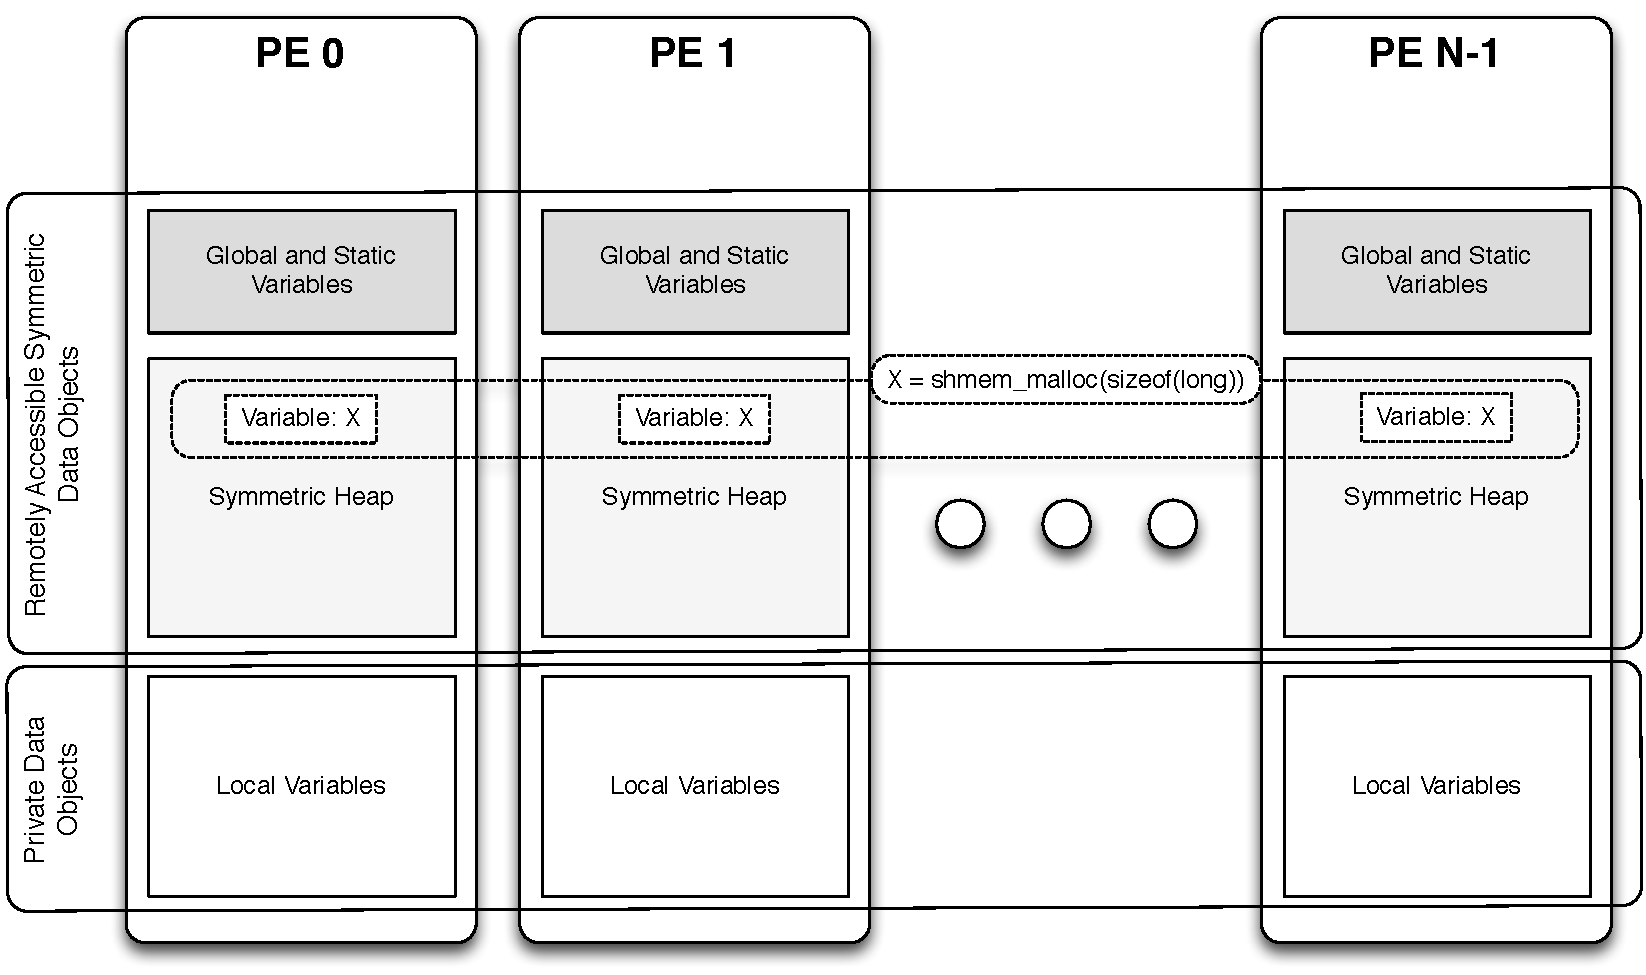
\includegraphics[width=0.95\textwidth]{figures/mem_model}
\caption{\openshmem Memory Model}
\label{fig:mem_model}
\end{figure}
%
An \openshmem program consists of data objects that are private to each \ac{PE}
and data  objects that are remotely accessible by all \acp{PE}. Private data
objects are stored in the local memory of each \ac{PE} and can only be accessed
by the \ac{PE} itself; these data objects cannot be accessed by other \acp{PE}
via \openshmem routines. Private data objects follow the memory model of
\Cstd. Remotely accessible objects, however, can be accessed by
remote \acp{PE} using \openshmem routines.  Remotely accessible data objects are
called \emph{Symmetric Data Objects}.  Each symmetric data object has a
corresponding object with the same name, type, and size on all \acp{PE} where that object is
accessible via the \openshmem \ac{API}\footnote{For efficiency reasons,
the same offset (from an arbitrary memory address) for symmetric data
objects might be used on all \acp{PE}. Further discussion about symmetric heap
layout and implementation efficiency can be found in section
\ref{subsec:shfree}}.  (For the definition of what is accessible, see the
descriptions for \FUNC{shmem\_pe\_accessible} and \FUNC{shmem\_addr\_accessible}
in sections \ref{subsec:shmem_pe_accessible} and
\ref{subsec:shmem_addr_accessible}.) Symmetric data objects accessed via typed and
type-generic \openshmem interfaces are required to be naturally aligned based on their type
requirements and underlying architecture.  In \openshmem the following kinds of
data objects are symmetric:
%
\begin{itemize}
\item Global and static \Cstd and \Cpp variables. These data objects must
  not be defined in a dynamic shared object (DSO).
\item \Cstd and \Cpp data allocated by \openshmem memory management routines
  (Section~\ref{sec:memory_management})
\end{itemize}

\openshmem dynamic memory allocation routines (e.g.,
\FUNC{shmem\_malloc}) allow collective allocation of \emph{Symmetric Data
Objects} on a special memory region called the \emph{Symmetric Heap}. The
Symmetric Heap is created during the execution of a program at a memory location
determined by the implementation. The Symmetric Heap may reside in different
memory regions on different \acp{PE}. Figure~\ref{fig:mem_model} shows how
\openshmem implements a \ac{PGAS} model using remotely accessible symmetric
objects and private data objects when executing an \openshmem program.
Symmetric data objects are stored on the symmetric heap or in the global/static
memory section of each \ac{PE}.

\subsection{Atomicity Guarantees}\label{subsec:amo_guarantees}

\openshmem contains a number of routines that perform atomic operations on
symmetric data objects, which are defined in Section \ref{sec:amo}.
The atomic routines
guarantee that concurrent accesses by any of these routines to the same
location and using the same datatype (specified in Tables~\ref{stdamotypes} and
\ref{extamotypes}) will be exclusive.
Exclusivity is also guaranteed when the target \ac{PE} performs a wait or test
operation on the same location and with the same datatype as one or more atomic
operations.
\openshmem atomic operations do not guarantee exclusivity in the following
scenarios, all of which result in undefined behavior.
\begin{enumerate}
    \item When concurrent accesses to the same location are performed using
        \openshmem atomic operations using different datatypes.
    \item When atomic and non-atomic \openshmem operations are used to access
        the same location concurrently.
    \item When \openshmem atomic operations and non-\openshmem operations (e.g.
        load and store operations) are used to access the same location
        concurrently.
\end{enumerate}
For example, during the execution of an atomic remote integer increment, i.e. \FUNC{shmem\_atomic\_inc},
operation on a symmetric variable \VAR{X}, no other \openshmem atomic operation
may access \VAR{X}.  After the increment, \VAR{X} will have increased its value
by \CONST{1} on the destination \ac{PE}, at which point other atomic operations
may then modify that \VAR{X}.  However, access to the symmetric object \VAR{X}
with non-atomic operations, such as one-sided \OPR{put} or \OPR{get} operations,
will invalidate the atomicity guarantees.

\cexample
    {The following \CorCpp example illustrates scenario 1.  In this example,
    different datatypes are used to access the same location concurrently,
    resulting in undefined behavior.  The undefined behavior can be resolved by
    using the same datatype in all concurrent operations.  For example, the
    32-bit value can be left-shifted and a 64-bit atomic OR operation can be
    used.}
    {./example_code/amo_scenario_1.c}

\cexample
    {The following \CorCpp example illustrates scenario 2.  In this example,
    atomic increment operations are concurrent with a non-atomic reduction
    operation, resulting in undefined behavior.  The undefined behavior can be
    resolved by inserting a barrier operation before the reduction.  The
    barrier ensures that all local and remote AMOs have completed before the
    reduction operation accesses $x$.}
    {./example_code/amo_scenario_2.c}

\cexample
    {The following \CorCpp example illustrates scenario 3.  In this example, an
    \openshmem atomic increment operation is concurrent with a local increment
    operation, resulting in undefined behavior.  The undefined behavior can be
    resolved by replacing the local increment operation with an \openshmem
    atomic increment.}
    {./example_code/amo_scenario_3.c}
